\documentclass{article}
\usepackage{graphicx}
\usepackage[dvipsnames,table]{xcolor}
\usepackage[utf8]{inputenc}
\usepackage{siunitx}
\usepackage[american,siunitx]{circuitikz}
\usepackage{amsmath}
\usepackage{svg}
\usepackage{booktabs}
\usepackage{float}
\usepackage{xparse, xfp}
\usepackage{multirow}
\usepackage{tikz}
\usepackage{karnaugh-map}
\usepackage{pdfpages}
\usepackage{pdflscape}
\usepackage{hyperref}

\newcommand{\overbar}[1]{\mkern 1.5mu\overline{\mkern-1.5mu#1\mkern-1.5mu}\mkern 1.5mu}
\hypersetup{
    colorlinks=true,
    linkcolor=blue,
    filecolor=magenta,      
    urlcolor=cyan,
}
\usepackage{caption} 

\makeatletter
\ctikzset{lx/.code args={#1 and #2}{ 
  \pgfkeys{/tikz/circuitikz/bipole/label/name=\parbox{1cm}{\centering #1  \\ #2}}
    \ctikzsetvalof{bipole/label/unit}{}
    \ifpgf@circ@siunitx 
        \pgf@circ@handleSI{#2}
        \ifpgf@circ@siunitx@res 
            \edef\pgf@temp{\pgf@circ@handleSI@val}
            \pgfkeyslet{/tikz/circuitikz/bipole/label/name}{\pgf@temp}
            \edef\pgf@temp{\pgf@circ@handleSI@unit}
            \pgfkeyslet{/tikz/circuitikz/bipole/label/unit}{\pgf@temp}
        \else
        \fi
    \else
    \fi
}}

\ctikzset{lx^/.style args={#1 and #2}{ 
    lx=#2 and #1,
    \circuitikzbasekey/bipole/label/position=90 } 
}

\ctikzset{lx_/.style args={#1 and #2}{ 
    lx=#1 and #2,
    \circuitikzbasekey/bipole/label/position=-90 } 
}
\makeatother

\captionsetup[table]{skip=10pt}

\usetikzlibrary{calc, automata, positioning}
%\usepackage[landscape]{geometry}
\renewcommand{\thesubsection}{\thesection.\alph{subsection}}
\newcommand{\equal}{=}
\newcommand{\greyrule}{\arrayrulecolor{black!30}\midrule\arrayrulecolor{black}}
\makeatletter
\newcommand\currcoor{\the\tikz@lastxsaved,\the\tikz@lastysaved}
\makeatother
\newcolumntype{:}{@{\hskip\tabcolsep\color{black!30}\vrule\hskip\tabcolsep}}

\ExplSyntaxOn
\NewExpandableDocumentCommand \groupify { O{\,\allowbreak} m m }
  { \jakob_groupify:nnn {#1} {#2} {#3} }
\cs_new:Npn \jakob_groupify:nnn #1 #2 #3
  { \__jakob_groupify_loop:nnw { 1 } {#2} #3 \q_recursion_tail {#1} \q_recursion_stop }
\cs_new:Npn \__jakob_groupify_loop:nnw #1 #2 #3
  {
    \quark_if_recursion_tail_stop:n {#3}
    \exp_not:n {#3}
    \int_compare:nNnTF {#1} = {#2}
      { \__jakob_groupify_sep:n }
      { \exp_args:Nf \__jakob_groupify_loop:nnw { \int_eval:n { #1+1 } } }
          {#2}
  }
\cs_new:Npn \__jakob_groupify_sep:n #1 #2 \q_recursion_tail #3
  {
    \tl_if_empty:nF {#2} { \exp_not:n {#3} }
    \__jakob_groupify_loop:nnw { 1 } {#1}
    #2 \q_recursion_tail {#3}
  }
\ExplSyntaxOff

\title{ECE 3300\\Digital Circuit Design Using Verilog\\\,\\Exercise 3}
\author{Choi Tim Antony Yung}
\begin{document}
\maketitle

\thispagestyle{empty}
\setcounter{page}{0}

\newpage

\section*{State Diagram}
\begin{figure}[H]
  \centering
  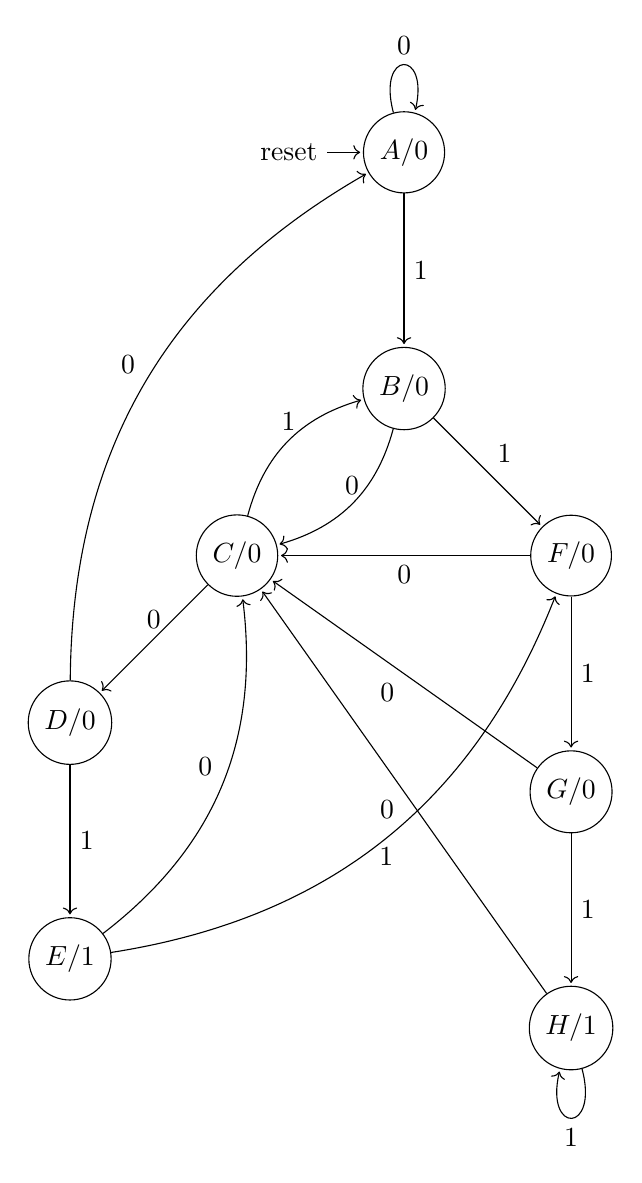
\begin{tikzpicture}[shorten >=1pt,node distance=3cm,on grid,auto] 
    \node[state,initial, initial text = reset] (A)   {$A/0$}; 
    \node[state] (B) [below =of A] {$B/0$}; 
    \node[state] (C) [below  left=of B] {$C/0$}; 
    \node[state] (D) [below  left=of C] {$D/0$}; 
    \node[state] (E) [below=of D] {$E/1$}; 
    \node[state] (F) [below right=of B] {$F/0$}; 
    \node[state] (G) [below =of F] {$G/0$}; 
    \node[state] (H) [below =of G] {$H/1$}; 
    \path[->]
     
     (A) edge [loop above] node {0} ()
         edge node {1} (B)
     (B) edge [bend left, above] node {0} (C)
         edge node {1} (F)
     (C) edge node [above] {0} (D)
          edge [bend left, above] node {1} (B)
     (D) edge [bend left] node {0} (A)
          edge node {1} (E)
     (E) edge [bend right] node {0} (C)
          edge [bend right, below] node {1} (F)
     (F) edge node {0} (C)
          edge node {1} (G)
     (G) edge node {0} (C)
          edge node {1} (H)
     (H) edge node {0} (C)
          edge [loop below] node {1} () 
     ;
  \end{tikzpicture}
\end{figure}
\newpage

\section*{State Table}
\begin{table}[H]
  \centering
  \begin{tabular}{c|c:c|c}
      \toprule
      Present&\multicolumn{2}{c|}{Next State}&Output\\
      State&$w=0$&$w=1$&$z$\\
      \midrule
      A&A&B&0\\
      B&C&F&0\\
      C&D&B&0\\
      D&A&E&0\\
      E&C&F&1\\
      F&C&G&0\\
      G&C&H&0\\
      H&C&H&1\\
      \bottomrule
  \end{tabular}
\end{table}

\section*{State-assigned Table}
\begin{table}[H]
  \centering
  \begin{tabular}{c:ccc|ccc:ccc|c}
      \toprule
      \multicolumn{4}{c|}{\multirow{2}{*}{Present State}}&\multicolumn{6}{c|}{Next State}&\multirow{2}{*}{Output}\\
      \multicolumn{4}{c|}{}&\multicolumn{3}{c:}{$w=0$}&\multicolumn{3}{c|}{$w=1$}&\\
      \greyrule
      \multicolumn{1}{c}{}&$y_2$&$y_1$&$y_0$&$Y_2$&$Y_1$&$Y_0$&$Y_2$&$Y_1$&$Y_0$&$z$\\
      \midrule
      A & 0&0&0 & 0&0&0 & 0&0&1 & 0\\
      B & 0&0&1 & 0&1&0 & 1&0&1 & 0\\
      C & 0&1&0 & 0&1&1 & 0&0&1 & 0\\
      D & 0&1&1 & 0&0&0 & 1&0&0 & 0\\
      E & 1&0&0 & 0&1&0 & 1&0&1 & 1\\
      F & 1&0&1 & 0&1&0 & 1&1&0 & 0\\
      G & 1&1&0 & 0&1&0 & 1&1&1 & 0\\
      H & 1&1&1 & 0&1&0 & 1&1&1 & 1\\
      \bottomrule
  \end{tabular}
\end{table}

\section*{Truth Table}
\begin{table}[H]
  \centering
  \begin{tabular}{cccc|cccc}
      \toprule
      $w$&$y_2$&$y_1$&$y_0$&$Y_2$&$Y_1$&$Y_0$&$z$\\
      \midrule
      0 & 0&0&0 & 0&0&0 & 0\\
      0 & 0&0&1 & 0&1&0 & 0\\
      0 & 0&1&0 & 0&1&1 & 0\\
      0 & 0&1&1 & 0&0&0 & 0\\
      0 & 1&0&0 & 0&1&0 & 1\\
      0 & 1&0&1 & 0&1&0 & 0\\
      0 & 1&1&0 & 0&1&0 & 0\\
      0 & 1&1&1 & 0&1&0 & 1\\
      1 & 0&0&0 & 0&0&1 & 0\\
      1 & 0&0&1 & 1&0&1 & 0\\
      1 & 0&1&0 & 0&0&1 & 0\\
      1 & 0&1&1 & 1&0&0 & 0\\
      1 & 1&0&0 & 1&0&1 & 1\\
      1 & 1&0&1 & 1&1&0 & 0\\
      1 & 1&1&0 & 1&1&1 & 0\\
      1 & 1&1&1 & 1&1&1 & 1\\
      \bottomrule
  \end{tabular}
\end{table}

\newpage

\section*{Karnaugh Maps}
\begin{table}[H]
  \begin{tabular}{cc}
    \begin{karnaugh-map}[4][4][1][$y_1y_0$][$wy_2$]
      \minterms{9,11,12,13,14,15}
      \implicant{13}{11}
      \implicant{12}{14}
    \end{karnaugh-map}
    &
    \begin{karnaugh-map}[4][4][1][$y_1y_0$][$wy_2$]
      \minterms{1,2,4,5,6,7,13,14,15}
      \implicant{5}{15}
      \implicant{7}{14}
    \end{karnaugh-map}
    \\
    $Y_2=\textcolor{red}{wy_0}+\textcolor{Green}{wy_2}=\textcolor{Purple}{w(y_2+y_0)}$
    &
    $Y_1
    =\textcolor{Red}{y_2y_0}
    +\textcolor{Green}{y_2y_1}
    +\textcolor{Purple}{\overbar{w}\left(y_2\oplus y_1 \oplus y_0\right)}
    $
    \\

    \quad\\ \\

    \begin{karnaugh-map}[4][4][1][$y_1y_0$][$wy_2$]
      \minterms{2,8,9,10,12,14,15}
      \implicantedge{12}{8}{14}{10}
      \implicantedge{2}{2}{10}{10}
    \end{karnaugh-map}
    &
    \begin{karnaugh-map}[4][4][1][$y_1y_0$][$wy_2$]
      \minterms{4,7,12,15}
    \end{karnaugh-map}
    \\
    $Y_0=\textcolor{red}{w\overbar{y_0}}
    +\textcolor{Green}{\overbar{y_2}y_1\overbar{y_0}}
    +\textcolor{Purple}{w\left(y_2\oplus y_1 \oplus y_0\right)}
    $
    &
    $z=\textcolor{Purple}{y_2\left(y_1\odot y_0\right)}$
    \\
  \end{tabular}
\end{table}

\newpage

\section*{Schematic}
\begin{figure}[H]
\centering
\begin{circuitikz}
  \draw
  (0,0) node[flipflop D](y2ff){}
  ++(1,-4) node[flipflop D](y1ff){}
  ++(1,-4) node[flipflop D](y0ff){}
  ;
  \draw[color=red]
  (y2ff.pin 6) node[below]{$y_2$} -- ++(0,4) -- ++ (-10,0) node[circ](y2){}
  (y2) -- ++(0,0.5) node[above]{$y_2$}
  (y2) -- ++(0,-15) coordinate(y2term)
  
  ;
  \draw[color=cyan]
  (y2) ++(0.5,-0.5) node[circ](y2n){}
  (y2n) -- (y2n|-y2) -- ++(0,0.5) node[above]{$\overbar{y_2}$}
  (y2n) -- (y2n|-y2term)
  (y2n) -- (y2n-|y2ff.pin 4) -- ++(0.5,0) -- (\currcoor|-y2ff.pin 4) -- (y2ff.pin 4) node[below]{$\overbar{y_2}$}
  ;
  \draw[color=green]
  (y2n) ++(0.5,-0.5) node[circ](y1){}
  (y1) -- (y1|-y2) -- ++(0,0.5) node[above]{$y_1$}
  (y1) -- (y1|-y2term)
  (y1) -- (y1-|y1ff.pin 6) -- (\currcoor|-y1ff.pin 6) -- (y1ff.pin 6) node[below]{$y_1$}
  ;
  \draw[color=magenta]
  (y1) ++(0.5,-0.5) node[circ](y1n){}
  (y1n) -- (y1n|-y2) -- ++(0,0.5) node[above]{$\overbar{y_1}$}
  (y1n) -- (y1n|-y2term)
  (y1n) -- (y1n-|y1ff.pin 4) -- ++(0.5,0) -- (\currcoor|-y1ff.pin 4) -- (y1ff.pin 4) node[below]{$\overbar{y_1}$}
  ;  
  \draw[color=blue]
  (y1n) ++(0.5,-0.5) node[circ](y0){}
  (y0) -- (y0|-y2) -- ++(0,0.5) node[above]{$y_0$}
  (y0) -- (y0|-y2term)
  (y0) -- (y0-|y0ff.pin 6) -- (\currcoor|-y0ff.pin 6) -- (y0ff.pin 6) node[below]{$y_0$}
  ;
  \draw[color=Yellow]
  (y0) ++(0.5,-0.5) node[circ](y0n){}
  (y0n) -- (y0n|-y2) -- ++(0,0.5) node[above]{$\overbar{y_0}$}
  (y0n) -- (y0n|-y2term)
  (y0n) -- (y0n-|y0ff.pin 4) -- ++(0.5,0) -- (\currcoor|-y0ff.pin 4) -- (y0ff.pin 4) node[below]{$\overbar{y_0}$}
  ;
  \draw
  (y2) ++(-1,0.5) node[above](w){$w$}
  (w) -- (w|-y2term)
  ;
  \draw[color = gray]
  (y2) ++(-0.5,0.5) node[above](wn){$\overbar{w}$}
  (wn) -- (wn|-y2term)
  ;
  \draw
  (y2ff.pin 1) node[and port, anchor = out](y2and){}
  (y2and.in 2) -- ++(0,-0.2) node[or port, anchor = out](y2or){}
  
  (y1ff.pin 1) -- (y1ff.pin 1-|y2ff.pin 1) node[or port, anchor = out, number inputs = 3](y1or){}
  (y1or.in 1) -- ++(0,0.8) node [and port, anchor = out](y1and1){}
  (y1or.in 2) -- ++(0,0) node [and port, anchor = out](y1and2){}
  (y1or.in 3) -- ++(0,-0.8) node [and port, anchor = out](y1and3){}
  
  (y0ff.pin 1) -- (y0ff.pin 1-|y2ff.pin 1) node[or port, anchor = out, number inputs = 3](y0or){}
  (y0or.in 1) -- ++(0,0.8) node [and port, anchor = out](y0and1){}
  (y0or.in 2) -- ++(0,0) node [and port,number inputs = 3, anchor = out](y0and2){}
  (y0or.in 3) -- ++(0,-0.8) node [and port, anchor = out](y0and3){}

  (y1and3.in 2) -- ++(0,-0.55) node[xor port,number inputs = 3, anchor = out](xor){} -- (y0and1.in 1)
  
  (y1-|y1ff.pin 6) ++(0.25,0) node [xnor port, anchor = in 1, rotate=90](xnor){}
  (xnor.out) -- ++(-0.5,0) node[and port, anchor = in 2, rotate=90](and){}
  (and.out) node[above]{$z$}
  ;

  \draw % w
  (y2and.in 1) -- (\currcoor-|w) node[circ]{}
  (y0and1.in 2) -- (\currcoor-|w) node[circ]{}
  (y0and3.in 1) -- (\currcoor-|w) node[circ]{}
  ;
  \draw[color=gray] % ~w
  (y1and3.in 1) -- (\currcoor-|wn) node[circ]{}
  ;
  \draw[color=red] % y2
  (y2or.in 1) -- (\currcoor-|y2) node[circ]{}
  (y1and1.in 1) -- (\currcoor-|y2) node[circ]{}
  (y1and2.in 1) -- (\currcoor-|y2) node[circ]{}
  (xor.in 1) -- (\currcoor-|y2) node[circ]{}
  (y2-|y2ff.pin 6) -- (\currcoor|-and.in 1) -- (and.in 1)
  ;
  \draw[color=cyan] % ~y2
  (y0and2.in 1) -- (\currcoor-|y2n) node[circ]{}
  ;
  \draw[color=green] % y1
  (y1and2.in 2) -- (\currcoor-|y1) node[circ]{}
  (y0and2.in 2) -- (\currcoor-|y1) node[circ]{}
  (xor.in 2) -- (\currcoor-|y1) node[circ]{}
  (y1-|y1ff.pin 6) -- (xnor.in 1)
  ;
  \draw[color=blue] % y0
  (y2or.in 2) -- (\currcoor-|y0) node[circ]{}
  (y1and1.in 2) -- (\currcoor-|y0) node[circ]{}
  (xor.in 3) -- (\currcoor-|y0) node[circ]{}
  (y0-|y0ff.pin 6) -- (\currcoor|-xnor.in 2) -- (xnor.in 2)
  ;
  \draw[color = Yellow] % ~y0
  (y0and2.in 3) -- (\currcoor-|y0n) node[circ]{}
  (y0and3.in 2) -- (\currcoor-|y0n) node[circ]{}
  ;
  \draw[color = brown] % clock
  (y2ff.pin 3) -- (\currcoor|-y2term) node[below](clk){clock}
  (y1ff.pin 3) -- (\currcoor-|clk) node[circ]{}
  (y0ff.pin 3) -- (\currcoor-|clk) node[circ]{}
  ;
\end{circuitikz}
\end{figure}

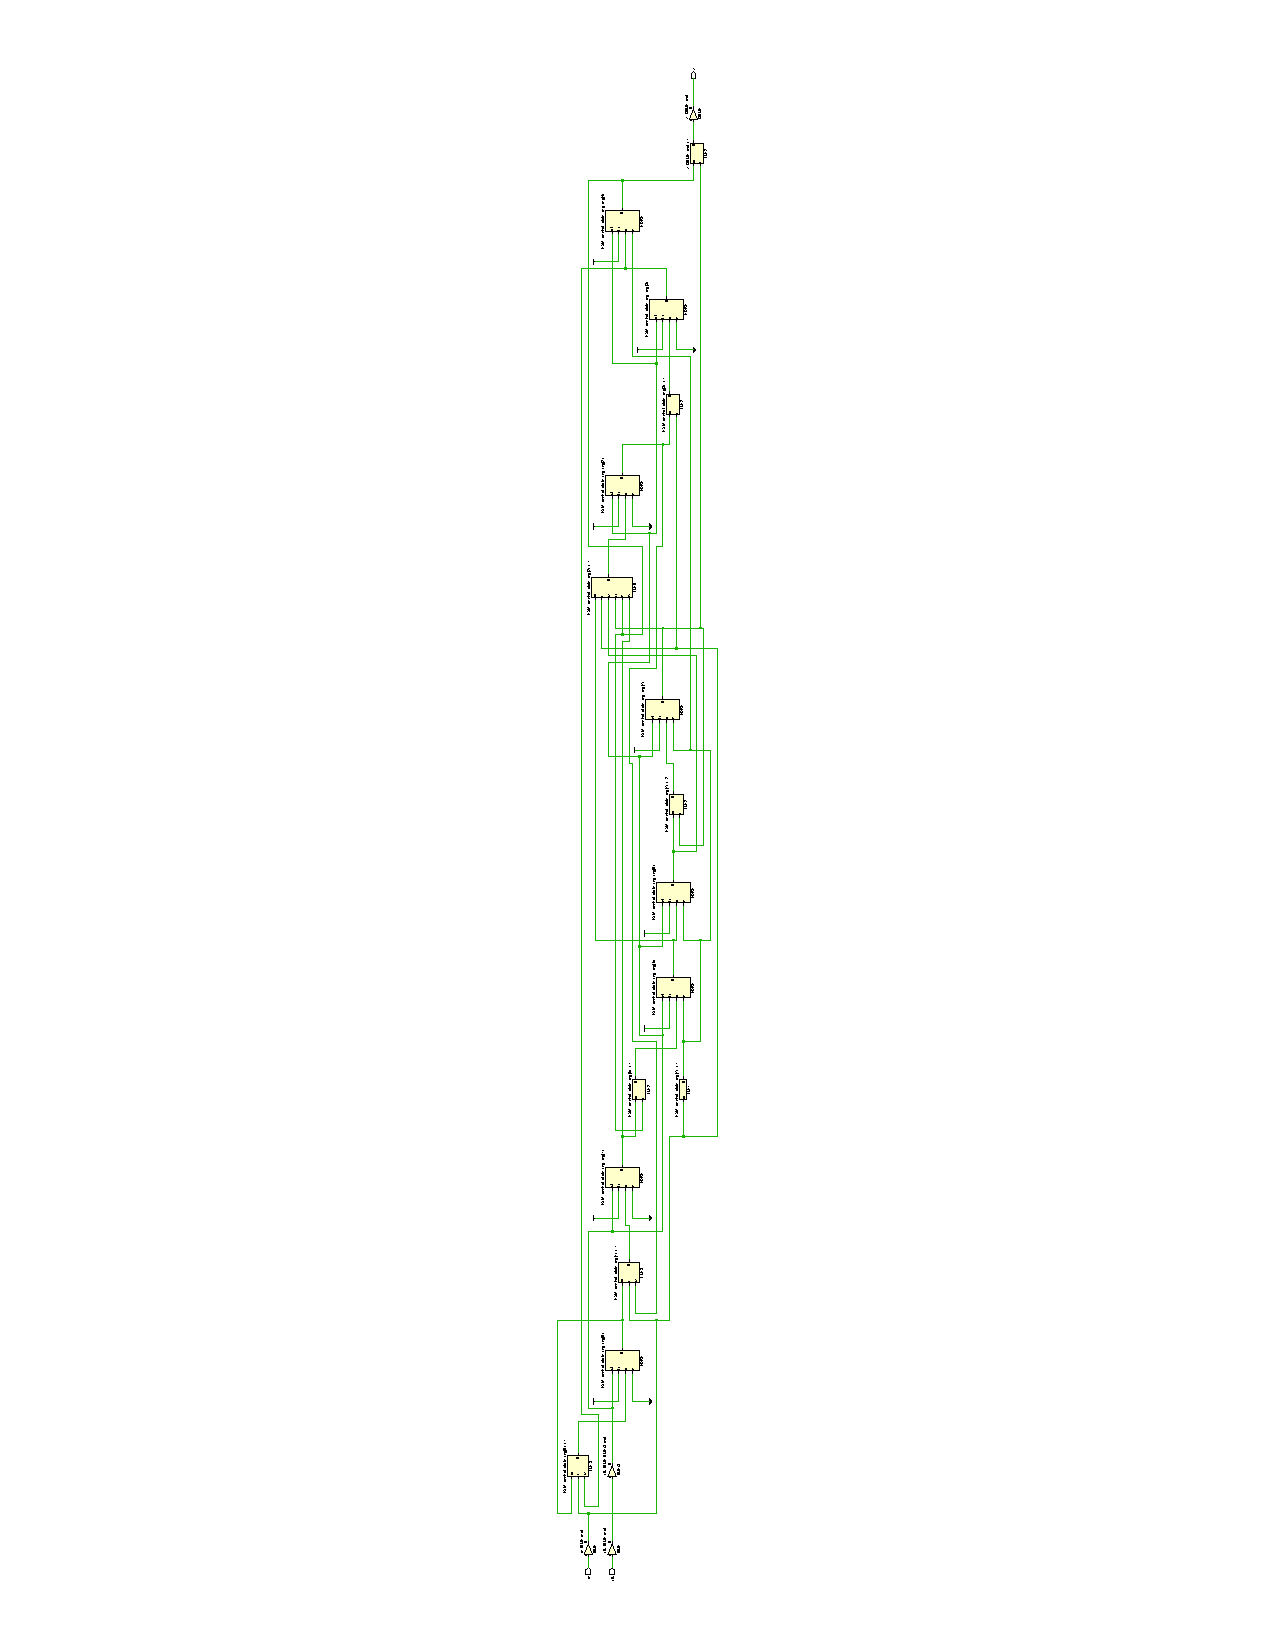
\includepdf{schematic.pdf}

\section*{Conclusion}
A significant difference between the two schematic is that the Vivado generated one use LUTs in contrast to logic gates. Also, the Vivado generated one have 8 flipflops instead of three.

\end{document}
